\chapter{Observations and  inconsistencies}\label{ch:inconst}

This chapter presents observations which were made about various features of \ecdar, including refinement, implementation, consistency and determinism checks. These observations help us to get a better understanding of features that we will implement. We are also going to show the inconsistencies which were found between \textsc{Ecdar} 0.10 and the theory and can be considered as flaws or bugs in the implementation. This is very important as all of the test cases of \jecdar are also tested in \ecdar 0.10, and therefore we must know which test cases we have to treat correctly with respect to theory. We will also explain why these kind of inconsistencies might be happening.

\section{An automaton does not refine itself}\label{sec:selfRef}
Based on the rules mentioned in Section \ref{sec:refRules}, the right side of the refinement has to be able to delay at least as much as the left side or more, which will always be the case in the same automaton, because of guards and invariants being the same. The same holds for outputs and inputs, since identical automata will always be able to comply with the corresponding output or input from the other side. However, if one would investigate \ecdar 0.10 in more depth they would notice that it provides the wrong result in some cases of self refinement. For example the case of Automaton \textbf{C1} from Figure \ref{fig:selfRefinementFail} is one of major inconsistencies of \ecdar 0.10 with the theory. If one would ask \ecdar 0.10 if \textbf{C1} <= \textbf{C1}, it would return that refinement fails. However, according to the theory, self refinement should always hold. If one was to create exactly the same automaton as \textbf{C1}, namely \textbf{C2}, the results would be exactly the same.

Nevertheless, creating the same automaton as \textbf{C1}, except having an additional reset $x=0$ on the input edge as in Figure \ref{fig:selfRefHold} would result in satisfying the refinement. Unfortunately, with the knowledge we have gathered, we cannot explain why \ecdar 0.10 treats it this way.
\begin{figure}
    \centering
    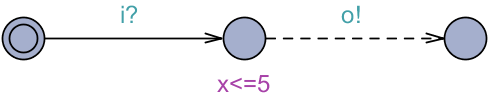
\includegraphics[scale = 0.7]{figures/selfRefFail.png}
    \caption{Automaton C1}
    \label{fig:selfRefinementFail}
\end{figure}

\begin{figure}
    \centering
    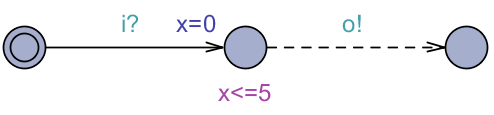
\includegraphics[scale = 0.7]{figures/selfRefHold.png}
    \caption{Automaton C3}
    \label{fig:selfRefHold}
\end{figure}

\section{No Specification as such}\label{sec:specification}
Based on \textcite{David:2010}, there exists a feature called specification, which we have described in \textcite{Jecdar:2019}. Throughout the year we have created multiple examples of specification checks in order to figure out how to properly implement it. However, we could not understand how exactly it works, since \ecdar 2.2 would return results which are completely incorrect according to the theory.

One of the observations that we were able to make when we started using \ecdar 0.10 was that asking for a specification check would return consistency results. We were able to see this only because \ecdar 0.10 returns an answer with a brief explanation, unlike \ecdar 2.2 which only returns true or false. This implies that \ecdar does not grant the possibility of checking for Specification.

Considering the fact that an automaton is a specification if each of its states are input-enabled and we are only working with input-enabled systems, then every automaton is a Specification. Therefore, there is no reason to have the feature Specification check as such.


\section{Partial input-enabledness}\label{sec:input-enabledness}
According to \textcite{David:2010}, "We restrict ourselves to input-enabled systems. This makes it impossible to reach an immediate deadlock state, where a component proposes an output that cannot be captured by the other component". This implies that \ecdar converts each automaton into a corresponding automaton which is input-enabled or treats it as if it was input-enabled. However, in some cases, \ecdar fails to treat an automaton as if it was input-enabled, which makes it inconsistent to the theory. We assume, that \ecdar imagines that there exist a loop of every input in every location, though it never tries to take these self loops first, which cuts out some of the solutions. 

For example, Figure \ref{fig:P4} and Figure \ref{fig:P5} represent two automata, \textbf{P4} and \textbf{P5} respectively and we deal with the case of \textbf{P4} <= \textbf{P5}. Refinement starts in state pair (\textbf{id0}, \textbf{id3}) where it checks if the right side can delay as much as the left side, which is true, then the left side checks if it has any outgoing outputs. Since there are no outputs, the right side checks for inputs, where it finds the input edge \textbf{i?}. Now one has to check if the left side can accept the same input at any given point when the right side is able to. This is true, since the right side can take that input edge at $[3;\infty]$, while the left side can do it at $[0;\infty]$. Then we arrive to the next state pair (\textbf{id0}, \textbf{id3}) with $[3;\infty]$, where we perform the delay check again, and it returns true. After the delay check one has to check for any outgoing outputs from the left side of the refinement, however given the fact that we arrive with the value of clock $y$ being $3$ or above, we are never able to take the \textbf{o!} output edge. The next step is to check if there are any input edges going from the right side and since there are none, the refinement according to \ecdar holds.
\begin{figure}
    \centering
    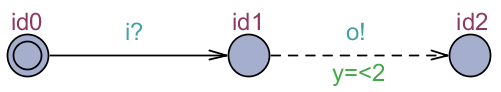
\includegraphics[scale = 0.7]{figures/P4.png}
    \caption{Automaton P4}
    \label{fig:P4}
\end{figure}
\begin{figure}
    \centering
    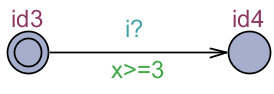
\includegraphics[scale = 0.7]{figures/P5.png}
    \caption{Automaton P5}
    \label{fig:P5}
\end{figure}

However, if one takes into consideration input-enabledness, there would be an additional path in the refinement. Figure \ref{fig:P4InputE} and Figure \ref{fig:P5InputE} provide a view of how \textbf{P4} and \textbf{P5} would look with the addition of input-enabledness. We are again concerned with the same case, \textbf{P4} <= \textbf{P5}, their state space exploration path can be seen at Figure \ref{fig:statePairsP4P5}. After checking for delays in the initial states, one can take a different path and do the self-loop on input \textbf{i?} on the right side, while on the left side taking the same edge as before, ending up in the state pair (\textbf{SP 1}) with the value of clock $x$ being $[0;3)$. Since our arrival time includes values below $2$, one can take the output edge \textbf{o!} on the left side, but the right side cannot comply and the refinement fails.

\begin{figure}
    \centering
    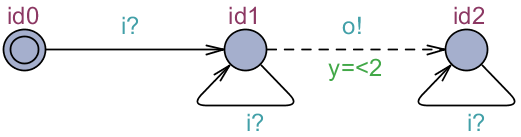
\includegraphics[scale = 0.7]{figures/P4InputEnabled.png}
    \caption{Automaton P4 input-enabled}
    \label{fig:P4InputE}
\end{figure}
\begin{figure}
    \centering
    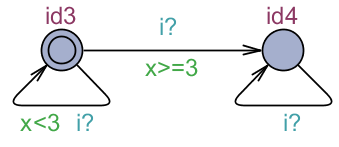
\includegraphics[scale = 0.7]{figures/P5InputEnabled.png}
    \caption{Automaton P5 input-enabled}
    \label{fig:P5InputE}
\end{figure}
\begin{figure}
\centering
\begin{tikzpicture}[thick,scale=0.9, every node/.style={scale=0.9}]
    \node[draw, anchor=south west,inner sep=0,  minimum width=3.7cm, minimum height=1.2cm] (box) at (0,0) {};
        \begin{scope}[ x={(box.south east)},y={(box.north west)}]
        \node[font=\Large] (a) at (box) {$\leq$};
        \node[align=center, left = 0.1mm of a] {\textbf{id0}\\$\bm{x[0;\infty)}$};
        \node[align=center, right = 0.1mm of a] {\textbf{id3}\\$\bm{x[0;\infty)}$};
        
        \node[align=center, above=0.25cm  of a](k)  {\textbf{SP 0}};
        \end{scope}
        
    \node[draw, anchor=south west,inner sep=0,  minimum width=3.7cm, minimum height=1.2cm] (box1) at (4,-2.5) {};
        \begin{scope}[ x={(box.south east)},y={(box.north west)}]
        \node[font=\Large] (a) at (box1) {$\leq$};
        \node[align=center, left = 0.1mm of a] {\textbf{id1}\\$\bm{x[0;\infty)}$};
        \node[align=center, right = 0.1mm of a] {\textbf{id3}\\$\bm{x[0;\infty)}$};
        \node[align=center, below= 1cm of a](k)  {\textbf{Refinement fails}};
        \draw [-latex,thick] (box1) --  node [right] {o!} (k) ;
        \node[align=center, above=0.25cm  of a](k)  {\textbf{SP 1}};
        \end{scope}
    \node[draw, anchor=south west,inner sep=0,  minimum width=3.7cm, minimum height=1.2cm] (box2) at (-4,-2.5) {};
        \begin{scope}[ x={(box.south east)},y={(box.north west)}]
        \node[font=\Large] (a) at (box2) {$\leq$};
        \node[align=center, left = 0.1mm of a] {\textbf{id1}\\$\bm{x[0;\infty)}$};
        \node[align=center, right = 0.1mm of a] {\textbf{id4}\\$\bm{x[0;\infty)}$};
        
        \node[align=center, above = 0.25cm of a](k)  {\textbf{SP 2}};
        \end{scope}
    \draw [-latex,thick] (box) --  node [right] {\hspace{0.25cm}i?} (box1) ;
    \draw [-latex,thick] (box) --  node [right] {\hspace{0.2cm}i?} (box2) ;

\end{tikzpicture}
\caption{State pairs of $P4<=P5$}
\label{fig:statePairsP4P5}
\end{figure}
To conclude, \ecdar gives the wrong results in cases like the ones mentioned above, since it does not take into consideration input-enabledness, even though it is stated that within this field input-enabledness should be assumed.

\section{Invariant bug}\label{sec:case1}
The case of refinement \textbf{T6} <= \textbf{T5}, whose components are illustrated in Figures \ref{fig:T6} and \ref{fig:T5}, holds according to \ecdar 0.10. In order to understand if this is correct, one has to take a closer look at how refinement works in this case. It starts in the initial states \textbf{id1} and \textbf{id4}, where the delay check is performed with positive results, afterwards the left side outputs with an \textbf{ro!}, while the right is capable of complying to it. The delay check is once again performed on the next state pair (\textbf{id1}, \textbf{id5}) - match. Now the right side is ready to move with input edge \textbf{ri?}, however the left side cannot comply with it, thus the refinement fails.

Surprisingly, if the invariant from location \textbf{id1} or \textbf{id2} (or even both) was removed, then the tool would show that the refinement fails. It is important to remember that according to the theory, in this example the invariants should not make a difference, since the refinement would still fail due to the left side not being able to comply with an input.
\begin{figure}
    \centering
    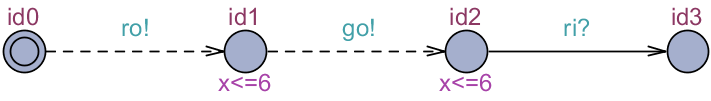
\includegraphics[scale = 0.7]{figures/T6.png}
    \caption{Automaton T6}
    \label{fig:T6}
\end{figure}
\begin{figure}
    \centering
    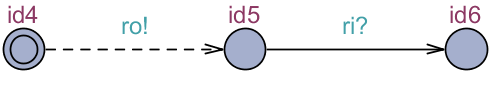
\includegraphics[scale = 0.7]{figures/T5.png}
    \caption{Automaton T5}
    \label{fig:T5}
\end{figure}
\section{Invariant bug nr2}\label{sec:invBug}
An important example in our observations was the refinement (\textbf{T1} || \textbf{T2}) <= \textbf{T3}, as it revealed a similar bug to the one mentioned in Section \ref{sec:case1}. This case is slightly different, since depending on the invariant value or its existence, the result is different. One can see the automata that are participating in this refinement in Figures \ref{fig:T1}, \ref{fig:T2} and \ref{fig:T3}. Figure \ref{fig:statePairsT1T2T3} provides the state space exploration of the refinement check on such automata, according to the theory. Each box provides the view of a state pair in the refinement. Inside the state pair, one can see a simplified version of the zones, which are represented as intervals. The green color marks the value in the interval which forces the remaining zones in the corresponding state pair to shrink. Lastly, the red color indicates places where the other side of the refinement cannot comply to the leading one.
 
\begin{itemize}
    \item (\textbf{State pair 0}) left side can delay up to 300, right side - match. Takes an \textbf{i!} edge.
    \item (\textbf{State pair 1}) left side can delay up to 1, right side - match. Delay check holds and takes \textbf{ri?} edge.
    \item (\textbf{State pair 2}) left side can delay up to 1, right side - match. Takes an \textbf{i!} self loop edge, automaton moves in composition as well with an \textbf{i?}.
    \item (\textbf{State pair 3}) left side can delay up to 1, right side - match. Cannot move anywhere anymore, since on the left side the invariant on \textbf{id2} is $x<=1$ and it blocks the possibility to move, the only output edge has a guard $x>=400$, while the right side does not have any input edges to force a movement.
    \item (\textbf{State pair 0}) left side can delay up to 300, right side - match. Takes an \textbf{ri?} edge - refinement move.
    \item (\textbf{State pair 4}) left side can delay up to 300, right side - 12, fail.
\end{itemize}


\begin{figure}
\centering

\begin{tikzpicture}[thick,scale=0.9, every node/.style={scale=0.9}]

    
    \node[draw, anchor=south west,inner sep=0,  minimum width=6.5cm, minimum height=1.2cm] (box) at (0,0) {};
        \begin{scope}[ x={(box.south east)},y={(box.north west)}]
        \node[align=center] (a) at (box) {\textbf{id0}\\$\bm{x[0;\infty)}$};
        \node[font=\Large, left = 0.1cm of a] {$\parallel$};
        \node[align=center, left = 0.7cm of a] {\textbf{id5}\\$\bm{x[0;$\colorbox{ForestGreen}{$300$}$]}$};
        \node[font=\Large, right = 0.1cm of a] {$\leq$};
        \node[align=center, right = 0.8cm of a] {\textbf{id8}\\$\bm{x[0;\infty)}$};
        
        \node[align=center, above=0.1mm  of a](k)  {\textbf{SP 0}};
        \end{scope}
        
    \node[draw, anchor=south west,inner sep=0,  minimum width=6.5cm, minimum height=1.2cm] (box1) at (4,-2.5) {};
        \begin{scope}[ x={(box1.south east)},y={(box1.north west)}]
        \node[align=center] (a) at (box1) {\textbf{id1}\\$\bm{x[0;\infty)}$};
        \node[font=\Large, left = 0.1cm of a] {$\parallel$};
        \node[align=center, left = 0.7cm of a] {\textbf{id5}\\$\bm{x[0;$\colorbox{ForestGreen}{$300$}$]}$};
        \node[font=\Large, right = 0.1cm of a] {$\leq$};
        \node[align=center, right = 0.8cm of a] {\textbf{id9}\\$\bm{x[0;$\colorbox{coralred}{$12$}$]}$};
        
        \node[align=center, above=0.1mm  of a](k)  {\textbf{SP 4}};
        \node[align=center, below= 0.5cm of a](k)  {\textbf{Refinement fails}};
        \draw [-latex,thick] (box1) --  node [right] {Delay check} (k) ;
        \end{scope}
    \node[draw, anchor=south west,inner sep=0,  minimum width=6.5cm, minimum height=1.2cm] (box2) at (-4,-2.5) {};
        \begin{scope}[ x={(box.south east)},y={(box.north west)}]
        \node[align=center] (a) at (box2) {\textbf{id0}\\$\bm{x[0;\infty)}$};
        \node[font=\Large, left = 0.1cm of a] {$\parallel$};
        \node[align=center, left = 0.7cm of a] {\textbf{id6}\\$\bm{x[0;$\colorbox{ForestGreen}{$1$}$]}$};
        \node[font=\Large, right = 0.1cm of a] {$\leq$};
        \node[align=center, right = 0.8cm of a] {\textbf{id8}\\$\bm{x[0;\infty)}$};
        \node[align=center, above=0.1mm  of a](k)  {\textbf{SP 1}};
        \end{scope}
    \node[draw, anchor=south west,inner sep=0,  minimum width=6.5cm, minimum height=1.2cm] (box3) at (-4,-5) {};
        \begin{scope}[ x={(box.south east)},y={(box.north west)}]
        \node[align=center] (a) at (box3) {\textbf{id1}\\$\bm{x[0;\infty)}$};
        \node[font=\Large, left = 0.1cm of a] {$\parallel$};
        \node[align=center, left = 0.7cm of a] {\textbf{id6}\\$\bm{x[0;$\colorbox{ForestGreen}{$1$}$]}$};
        \node[font=\Large, right = 0.1cm of a] {$\leq$};
        \node[align=center, right = 0.8cm of a] {\textbf{id9}\\$\bm{x[0;12]}$};
        \node[align=center, above left=0.1cm  of a](k)  {\textbf{SP 2}};
        \end{scope}
    \node[draw, anchor=south west,inner sep=0,  minimum width=6.5cm, minimum height=1.2cm] (box4) at (-4,-7.5) {};
        \begin{scope}[ x={(box.south east)},y={(box.north west)}]
        \node[align=center] (a) at (box4) {\textbf{id2}\\$\bm{x[0;500]}$};
        \node[font=\Large, left = 0.1cm of a] {$\parallel$};
        \node[align=center, left = 0.7cm of a] {\textbf{id6}\\$\bm{x[0;$\colorbox{ForestGreen}{$1$}$]}$};
        \node[font=\Large, right = 0.1cm of a] {$\leq$};
        \node[align=center, right = 0.8cm of a] {\textbf{id9}\\$\bm{x[0;12]}$};
        \node[align=center, above left=0.1cm  of a](k)  {\textbf{SP 3}};
        \end{scope}
    \draw [-latex,thick] (box) --  node [right] {\hspace{0.25cm}ri?} (box1) ;
    \draw [-latex,thick] (box) --  node [right] {\hspace{0.2cm}i!} (box2) ;
    \draw [-latex,thick] (box2) --  node [right] {ri?} (box3) ;
    \draw [-latex,thick] (box3) --  node [right] {i!} (box4) ;
    
\end{tikzpicture}
\caption{State pairs of $T1||T2<=T3$}
\label{fig:statePairsT1T2T3}
\end{figure}
Nevertheless, performing a {refinement} check in \ecdar 0.10 produces a different result, which is inconsistent to the theory, namely that it holds. In order to explain why \ecdar 0.10 ends up having different results, we need to take a look at the transition going from location \textbf{id5} to \textbf{id6}. Having the invariant $x<=1$ on location \textbf{id5} would tighten the invariant on \textbf{id5}, since one could never arrive to \textbf{id6} with values above $1$. Thus the delay check in state pair ((\textbf{id1}, \textbf{id5}), \textbf{id9}) would never fail. It is important to note that this is simply a guess, since we cannot be certain why \ecdar 0.10 treats this case differently than the theory.

Another interesting phenomenon happens when removing the invariant from location \textbf{id5}. According to the theory the results should be the same, since without an invariant it would fail in the same state. However, \ecdar 0.10 outputs a different result, stating that the refinement fails. Unfortunately, we have not derived a proper explanation for why \ecdar 0.10 treats this differently than the case with the invariant, which clearly violates the delay check of the refinement.
\begin{figure}
    \centering
    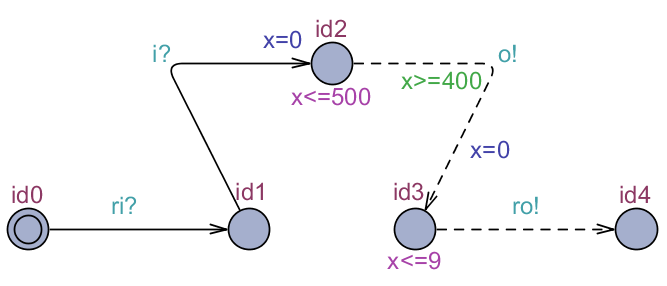
\includegraphics[scale = 0.7]{figures/T1.png}
    \caption{Automaton T1}
    \label{fig:T1}
\end{figure}
\begin{figure}
    \centering
    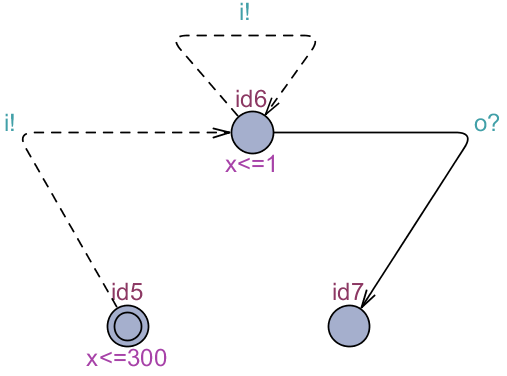
\includegraphics[scale = 0.7]{figures/T2.png}
    \caption{Automaton T2}
    \label{fig:T2}
\end{figure}
\begin{figure}
    \centering
    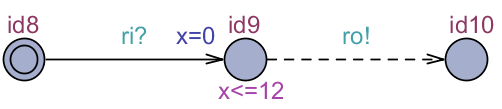
\includegraphics[scale = 0.7]{figures/T3.png}
    \caption{Automaton T3}
    \label{fig:T3}
\end{figure}
\section{Signature check}\label{sec:signatureCheck}
We have observed that \ecdar performs some sort of signature check. Having additional outputs on the left side, while the right side has them only in the signature but not in the component itself breaks the refinement. The same applies for the inputs, having an additional input on the right side, while the left side does not have it even in the signature, the refinement holds. On the other hand, if one would add such an input to the signature, the refinement would fail. The refinement of \textbf{N3<=N4}, whose components can be seen in Figures \ref{fig:N3} and \ref{fig:N4} shows the case where, according to \ecdar, having an input only in the signature of the automaton which is present on the right side leads to the failure of the refinement. However, according to the theory, all the components are input-enabled, which implies that the left side should be able to perform the "imaginary self loop" on the missing input \textbf{i2?}. 

\begin{figure}
    \centering
    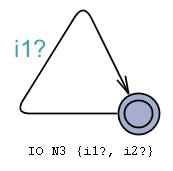
\includegraphics[scale = 0.7]{figures/N3.png}
    \caption{Automaton N3}
    \label{fig:N3}
\end{figure}
\begin{figure}
    \centering
    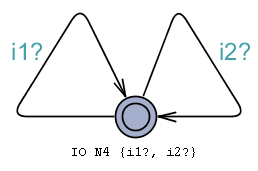
\includegraphics[scale = 0.7]{figures/N4.png}
    \caption{Automaton N4}
    \label{fig:N4}
\end{figure}

\section{Types of consistency check}\label{sec:minConsistency}
In the beginning we were only aware of the existence of one type of consistency, which needs to check the whole automaton in order to make sure it is consistent. However, throughout our project an observation have been made, that there exist different types of consistencies: 
\begin{itemize}
    \item Least fixpoint consistency
    \item Greatest fixpoint consistency
    \item Full consistency
\end{itemize}
This semester we are only going to handle the least fixpoint and the full consistency. The full consistency has to check the whole automaton in order for it to return a result. On the other hand, the least fixpoint consistency can prune some of the edges in order to find the smallest part of the automaton that is consistent. It can prune all the outputs, since they are controllable, unlike inputs which can neither be controlled nor pruned. Opposite to least fixpoint consistency, the greatest fixpoint consistency finds the biggest part of an automaton, which is consistent.

\ecdar provides only one type of consistency - the least fixpoint consistency check. Consider the example in Figure \ref{fig:G21}, which starts in the initial location, where there is an output edge going from it. Since it is an output, we can prune the rest of the automaton and have the least fixpoint consistency. On location \textbf{id2} there is an invariant and there are no output edges going from it that could solve the problem. However, since the rest of the automaton was pruned, this does not matter anymore.
\begin{figure}
    \centering
    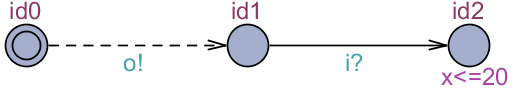
\includegraphics[scale = 0.7]{figures/G21.png}
    \caption{Automaton G21}
    \label{fig:G21}
\end{figure}

\section{Determinism bug}\label{sec:determBug}
An important aspect to remember is that all automata must be deterministic. If there are multiple outgoing edges from the same location with the same action, a determinism check has to be made in order to ensure that there exists only one path at any given point in time. \ecdar always performs a determinism check before running queries and it appears as though it is always able to determine correctly if an automaton is deterministic.

In spite of this, we have succeeded to find a case where \ecdar fails at the determinism check. Consider Figure \ref{fig:P8}, where \ecdar states that this automaton is deterministic. In this example there are three different edges from the initial location \textbf{id0}. In the case of the two edges that lead to location \textbf{id2}, the intervals in which these edges can be traversed do not overlap, but in the case of the third edge which leads to location \textbf{id1}, the interval overlaps with one of the other edges. Thus, the determinism check should fail. It seems like in the cases where there are multiple edges going from one location to another one, they are being excluded from further determinism checks in \ecdar.
\begin{figure}
    \centering
    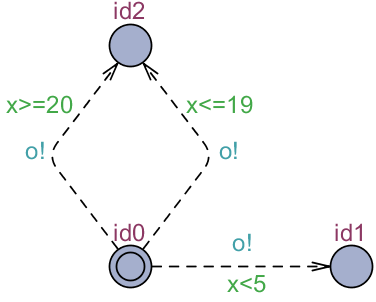
\includegraphics[scale = 0.7]{figures/P8.png}
    \caption{Automaton P8}
    \label{fig:P8}
\end{figure}
\section{Global time correspondence}\label{sec:globalTime}
Another important observation that was made was about \ecdar's global time correspondence. Dealing with time in this field is important, so it is crucial to understand as much as possible about it. One has to keep in mind that arriving at a certain time in two automata that are in a refinement relation will always result in being at the same time in accordance with its minimum and maximum values.

In order to understand this better, one should take a look at the relation of \textbf{K5} <= \textbf{K6}, which is represented in Figures \ref{fig:K5} and \ref{fig:K6}. The arrival time in \textbf{id1} is $0$, because of the reset and the arrival time in \textbf{id4} is $5$. The time correspondence is simple in this case, since in both automata we have only one value. However, in the case of the arrival times in \textbf{id2} and in \textbf{id5}, they will end up being intervals, $[0;10]$ and $[5;15]$, respectively. The actual arrival time in the previously mentioned state pair would be somewhere in the middle, but at the same point in time, given the minimum or maximum values of each interval. It is impossible to arrive in such a state pair with one of the automata being at its maximum arrival time and the other one at its minimum. The reasoning behind this is that time always moves at the same rate and it cannot be frozen in any of the automata.
\begin{figure}
    \centering
    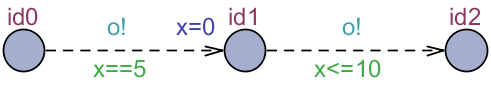
\includegraphics[scale = 0.7]{figures/K5.png}
    \caption{Automaton K5}
    \label{fig:K5}
\end{figure}
\begin{figure}
    \centering
    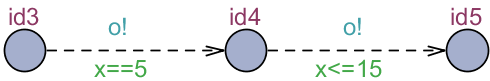
\includegraphics[scale = 0.7]{figures/K6.png}
    \caption{Automaton K6}
    \label{fig:K6}
\end{figure}


\section{Exploration of refinement with input-enabledness}\label{sec:case2}
After analysing the refinement of \textbf{T9} <= \textbf{T8}, which is illustrated in Figures \ref{fig:T8} and \ref{fig:T9}, valuable information of how refinement works in \ecdar can be derived. It starts in the initial locations \textbf{id4} and \textbf{id0}, where the delay check is satisfied. Afterwards, the right side makes a move on input edge \textbf{i1?}, while the left side is able to comply. Now the left side has only one move, which is a common input \textbf{i2?}, while the left side also has one move, namely common output \textbf{o!}. Here the refinement check is complete and \ecdar returns true, which implies that the rest of the automaton is not explored, since refinement would fail at a later point.
\begin{figure}
    \centering
    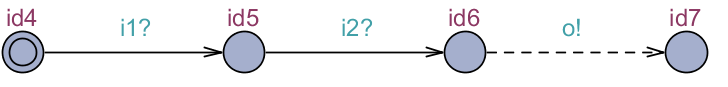
\includegraphics[scale = 0.7]{figures/T9.png}
    \caption{Automaton T9}
    \label{fig:T9}
\end{figure}
\begin{figure}
    \centering
    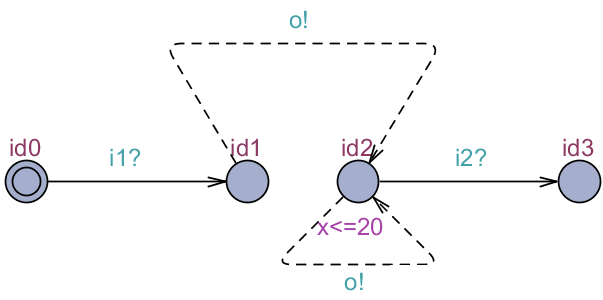
\includegraphics[scale = 0.7]{figures/T8.png}
    \caption{Automaton T8}
    \label{fig:T8}
\end{figure}
According to the rules of refinement, the left side can force to move on outputs and the right side can do the same on inputs. The fact that \ecdar stops the exploration at this point is in accordance with the theory, since it is not stated what happens when the only possible movements are with the input from the left and with the output from the right. However, if we take into consideration input-enabledness, everything changes. Now, according to the theory the refinement should fail. The state space exploration is provided in Figure \ref{fig:statePairsT9T8}, which is performed in accordance to the theory.

The refinement check begins in state pair 0, where the right side can comply to the delay check. Both sides move with an input edge \textbf{i1?}. In state pair 1 the delays match and now we may perform a self loop on location \textbf{id1} on input \textbf{i2?}, while the left side can comply to it. Now the left side is the leading one with an output edge \textbf{o!}, which can be traversed with $\bm{x\in[0;\infty]}$, while the right side cannot comply to it, since its output edge \textbf{o!} can be traversed only with $\bm{x\in[0;20]}$, thus the refinement fails.

\begin{figure}
\centering
\begin{tikzpicture}[thick,scale=0.9, every node/.style={scale=0.9}]
    \node[draw, anchor=south west,inner sep=0,  minimum width=3.7cm, minimum height=1.2cm] (box) at (0,0) {};
        \begin{scope}[ x={(box.south east)},y={(box.north west)}]
        \node[font=\Large] (a) at (box) {$\leq$};
        \node[align=center, left = 0.1mm of a] {\textbf{id4}\\$\bm{x[0;\infty)}$};
        \node[align=center, right = 0.1mm of a] {\textbf{id0}\\$\bm{x[0;\infty)}$};
        
        \node[align=center, above left=0.25cm  of a](k)  {\textbf{SP 0}};
        \end{scope}
        
    \node[draw, anchor=south west,inner sep=0,  minimum width=3.7cm, minimum height=1.2cm] (box1) at (0,-2.5) {};
        \begin{scope}[ x={(box.south east)},y={(box.north west)}]
        \node[font=\Large] (a) at (box1) {$\leq$};
        \node[align=center, left = 0.1mm of a] {\textbf{id5}\\$\bm{x[0;\infty)}$};
        \node[align=center, right = 0.1mm of a] {\textbf{id1}\\$\bm{x[0;\infty)}$};
        
        \node[align=center, above left=0.25cm  of a](k)  {\textbf{SP 1}};
        \end{scope}
    \node[draw, anchor=south west,inner sep=0,  minimum width=3.7cm, minimum height=1.2cm] (box2) at (0,-5) {};
        \begin{scope}[ x={(box.south east)},y={(box.north west)}]
        \node[font=\Large] (a) at (box2) {$\leq$};
        \node[align=center, left = 0.1mm of a] {\textbf{id6}\\$\bm{x[0;\infty)}$};
        \node[align=center, right = 0.1mm of a] {\textbf{id1}\\$\bm{x[0;\infty)}$};
        
        \node[align=center, above left=0.25cm  of a](k)  {\textbf{SP 2}};
        \node[align=center, below= 1cm of a](k)  {\textbf{Refinement fails}};
        \draw [-latex,thick] (box2) --  node [right] {o!} (k) ;
        \end{scope}

    \draw [-latex,thick] (box) --  node [right] {i1?} (box1) ;
    \draw [-latex,thick] (box1) --  node [right] {i2?} (box2) ;
\end{tikzpicture}
\caption{State pairs of $T9<=T8$}
\label{fig:statePairsT9T8}
\end{figure}


\section{Treatment of syncs as outputs}\label{sec:case3}
The refinement which is illustrated in Figure \ref{fig:P8||P9<=P10} holds in \ecdar. However, according to the theory, in this case it should not even pass the signature check. The reasoning behind this is that the left side cannot have an action \textbf{i} being an input and an output at the same time, while on the left it exists as an input. If on the right side \textbf{i} would be an output  instead of an input, then the refinement would hold. This happens because syncs are treated as outputs, therefore \textbf{i} would be an output on both sides and the signature check would pass.
\begin{figure}
\centering
\begin{tikzpicture}[thick,scale=0.7, every node/.style={scale=0.7}]
    \node[anchor=south west,inner sep=0] (image) at (0,0)
    {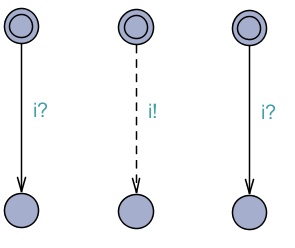
\includegraphics{figures/P8CompP9RefP10.png}};
    \begin{scope}[x={(image.south east)},y={(image.north west)}]
        
        \node[font=\Large] at (0.65,0.5) {$\Scale[2]{{\leq}}$};
        \node[font=\Large] at (0.27,0.5) {$\Scale[2]{{\parallel}}$};
    \end{scope}
\end{tikzpicture}
\caption{Refinement which should not pass the signature check} \label{fig:P8||P9<=P10}
\end{figure}